\documentclass[11pt]{article}
\usepackage{acl2016}
\usepackage{times}
\usepackage{url}
\usepackage{latexsym}
\aclfinalcopy% Uncomment this line for the final submission

\usepackage{xcolor,colortbl}
\usepackage{color}
\usepackage{caption}
\usepackage{subcaption}
\usepackage{graphicx}
\usepackage{booktabs}

\definecolor{Gray}{gray}{0.85}
\definecolor{LightCyan}{rgb}{0.9, 0.9, 0.98}


%\aclfinalcopy % Uncomment this line for the final submission
%\def\aclpaperid{***} %  Enter the acl Paper ID here

%\setlength\titlebox{5cm}
% You can expand the titlebox if you need extra space
% to show all the authors. Please do not make the titlebox
% smaller than 5cm (the original size); we will check this
% in the camera-ready version and ask you to change it back.

\newcommand\BibTeX{B{\sc ib}\TeX}

\usepackage{amsmath,lipsum}
\newcommand{\mypm}{\mathbin{\smash{%
\raisebox{0.35ex}{%
            $\underset{\raisebox{0.5ex}{$\smash -$}}{\smash+}$%
            }%
        }%
    }%
}

\title{Predicting Reactions to Blog Headlines}

\author{Rel Guzman, Jose Eduardo Ochoa-Luna, Laura Cruz-Quispe, Elizabeth Vera-Cervantes \\
Universidad Nacional de San Agustin \\
Arequipa, Peru \\
  {\tt \{r.guzmanap,eduardo.ol,lvcruzq,elizavvc\}@gmail.com} \\}


\date{}

\begin{document}
\maketitle
\begin{abstract}

This paper describes some experiments carried out to measure sentiment, which we call emotional reaction, on blog headlines. We analyze a text corpus of titles from Facebook entries or posts linking to a website. These titles are basically headlines and we study them to understand the relationship between article headlines and the self-reported reactions of the articles' readers. We utilize the recently launched feature, Facebook reactions that enable people to express their emotional reactions with five emojis. These reactions and headlines are gathered from different fan-pages, we analyze them, make an exploratory data analysis and present preliminary results of a reaction predictor.

\end{abstract}


\section{Introduction}

Sharing online content is an integral part of modern life, this is somewhat related with social transmissions which are driven in part by arousal, this hypothesis suggests why content that evokes more of certain emotions is more shared~\cite{berger2011arousal}. We analyze a text corpus of titles from Facebook entries or posts linking to a website. These titles are headlines and we study them to understand the relationship between article headlines and the self-reported reactions of the articles' readers. We utilize the recently launched feature, Facebook reactions that enable people to express their emotional reactions with five emojis. Then, we propose a simple approach to predict people's reactions to textual content by analyzing emotional reactions. 

As with sentiment detection, this problem is treated as a simple classification problem and achieve very high accuracy by employing various machine learning algorithms. Although, simple classification provides limited information about sentiment, that's the reason we also used another type of classifier with which we are able to compute the probability of each reaction.

A reaction is predicted using a predictive model consisting of Term frequency – Inverse Document Frequency (TF-IDF), a Linear Support Vector Classifier (SVC) and a Stochastic Gradient Descent (SGD) algorithm. Preliminary experiments were run on 14 fan-pages forming a big dataset, and results show suitability of our approach. 

The paper is organized as follow: In Section 2 related work is described, next in Section 3 the dataset is described, then our proposal is described in Section 4. We provide experiments and results of the proposed method in Section 5. Finally, we provide concluding remarks in Section 6. The source code to reproduce this paper is available online~\footnote{https://github.com/rgap/simbig2016-facebook-reactions}.


\section{Related Work}

Among recent studies on sentiment analysis applied on Facebook, most of them analyze public posts shared by users \cite{rastogi2014sentiment}, \cite{gao2015more}. Taking into account information such as a text messages, comments, likes. But, currently none of them have studied its new feature, ``reactions'', neither how a reaction could affect the popularity of content. Predicting the popularity of social media content has been approached from many angles. Some have even been using measurements of items at their early popularity applying survival analysis \cite{lee2010approach}. Typically, the goal of those researches is to predict the popularity like the number of comments that will be generated by an article based on its content, or how long will it be popular.

A common line of research focuses on predicting the spread of ideas and information using content, topology and linguistic features. On twitter, authors tend to pay special attention to sentiment indicators from the content of tweets, including counts of emoticons and strength of word-level sentiments \cite{kong2014predicting}.

There are studies that suggest that content that evokes either high-arousal positive emotions (awe) or negative emotions (anger or anxiety) tends to be more viral \cite{berger2013emotion}. Therefore, a headline popularity can also be measured according to what emotion, sentiment, or reaction it produces. And, there are also recent studies that deal with sentiment analysis on headlines and short-texts \cite{nassirtoussi2015text}. 


\section{Dataset}

All posts were extracted using the Facebook Graph API, from 14 fan-pages of popular websites about news, science, and entertainment: Buzzfeed, 9gag, Boredpanda, Mashable, Unilad, CNN, CNN international, DailyMail, FoxNews, HuffingtonPost, New York Times, IFeakingLoveScience, IMDB, and Natgeo. And because Facebook reactions were launched after February 2016, the dataset was sliced so that it only contains samples within ``2016-04-01'' and ``2016-07-31''. We obtained a dataset of 9072 samples.

\subsection{Reactions}

After an administrator posts a link directing to a website article on Facebook, a thumbnail is generated which contains: image, description, and a title. A user is redirected to the article after clicking on the thumbnail then reads it, goes back to Facebook and gives it a reaction, or probably does it before even clicking on it. Therefore, we analyzed a text corpus of titles from Facebook posts. These titles are like news headlines and we studied them to understand the relationship between them and the self-reported reactions of the articles' readers. We utilized the recently launched feature, Facebook reactions that enable people to express their emotional reactions with one of five emojis: ``love'', ``haha'', ``wow'', ``sad'', and ``angry''. We selected BuzzFeed as one of the fan-pages due to a feature its website has, a registered user is allowed to comment on an article with a type of reaction defined by the website, the types of reactions are: ``love'', ``lol'', ``fail'', ``wtf'', among others but these are the most voted.

To predict a specific reaction to a headline, we defined a target $y$ which is the most voted reaction among only the reactions, not considering the number of likes. Furthermore, we added it to the dataset only if its number of votes was higher than 75\% of the total number of votes, so we make sure people reacted in just one way, because some of them could have the same number of votes per reaction. The number of reaction votes per reaction sorted by their means is shown in Figure \ref{fig:boxplot}. This diagram doesn't tell too much only that even taking into account many fan-pages, the sad reaction isn't the most voted. We took away the headlines with a most voted reaction with less than $200$ votes.

\begin{figure}[ht!]
\centering
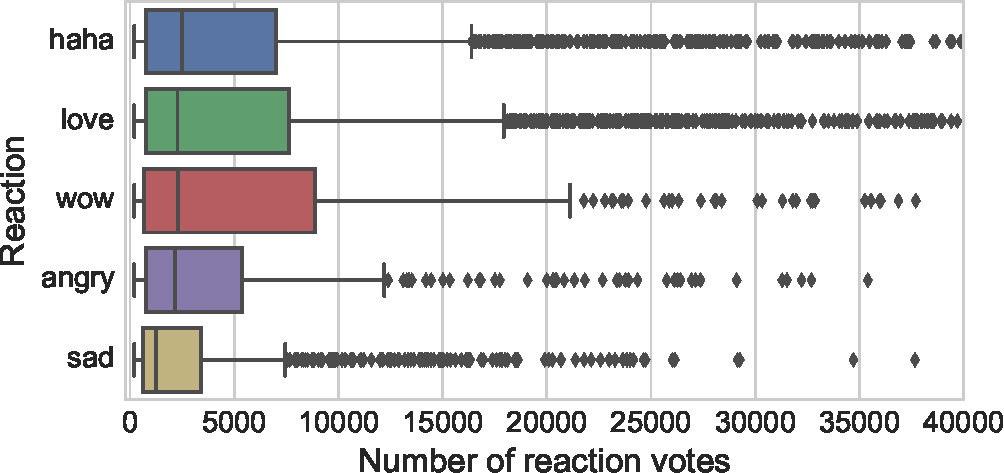
\includegraphics[width=1.0\columnwidth]{../3_notebooks/notebook_figures/boxplots_fblike_reactions.pdf}
\caption{Box plots sorted base on median value, showing the number of reactions votes (total number of reaction votes) per reaction and outliers. }
\label{fig:boxplot}
\end{figure}

A correlation matrix is shown in Figure \ref{fig:corr}, it shows how the ``number of reactions'', ``comments'', ``shares'', ``likes'' and the reactions correlate among them.

\begin{figure}[ht!]
\centering
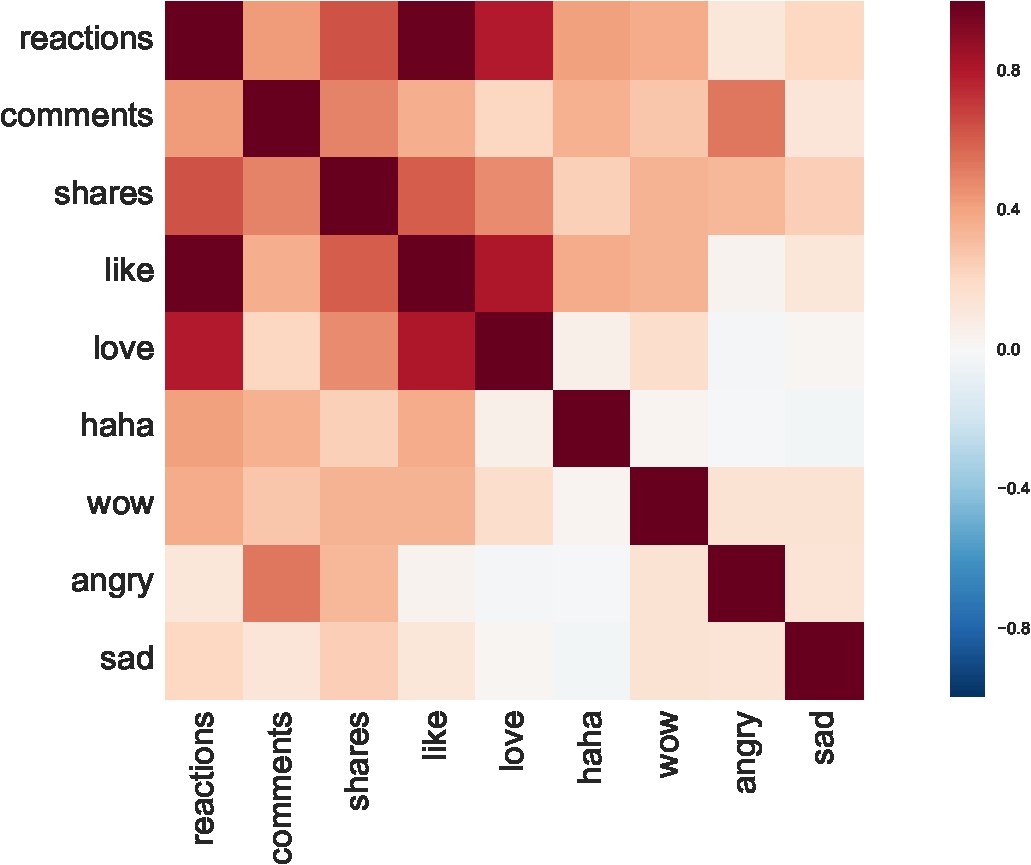
\includegraphics[width=1.0\columnwidth]{../3_notebooks/notebook_figures/corr_mat.pdf}
\caption{Correlation matrix showing how ``love'' is more linearly correlated to the number of reactions and shares. An interesting insight shows how ``angry'' is more correlated to the number of comments, showing that people comment more when dealing with controversial topics.}
\label{fig:corr}
\end{figure}

\subsection{Headlines}

We needed to get features to predict a specific reaction, these features were extracted from the headlines. Some of the headlines are less specific to a special date or event like ``numbered lists'' also known as ``listcicles'' like:
\begin{itemize}
 \item 24 Heartbreaking TV Moments That Made You Cry Your Eyes Out.
 \item 27 Surreal Places To Visit Before You Die.
\end{itemize}

We selected BuzzFeed also because it creates these types of posts, but not so many to take only BuzzFeed into account. A predictor of these types of headlines would have been easier to optimize, but it is harder to know if a title is one of these, at least not automatically, also we wanted to make it more general. That's the reason we gathered data from many fan-pages.

Then, we figured out the dataset from ``buzzfeed'' contained english and spanish headlines, spanish ones were taken away from the corpus. The headlines were tokenized and we took normal words, abbreviations and words with internal hyphens/apostrophe. We took Unicode words like ``Über'' and represented them in US-ASCII characters so that it becomes ``Uber''. More preprocessing is done like profanity censorship converting every bad word in the token ``badword''. Then we removed common and some special stopwords, we did lemmatization and stemming.

A histogram with number of headlines per reaction in descending order is shown in Figure \ref{fig:hist}, it shows that the dataset is imbalanced.

\begin{figure}[ht!]
\centering
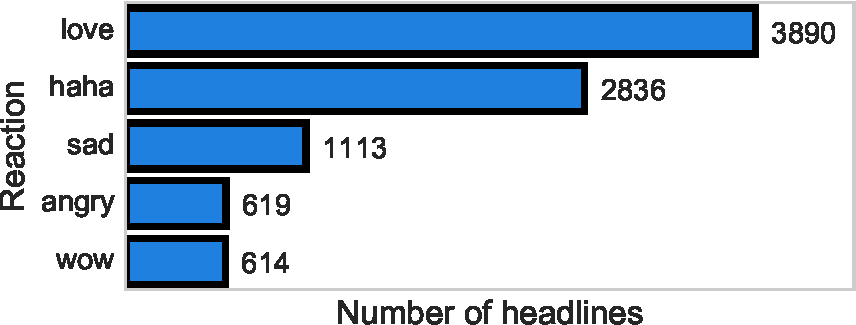
\includegraphics[width=1.0\columnwidth]{../3_notebooks/notebook_figures/histogram_reactions.pdf}
\caption{Final histogram of the dataset showing the number of samples (headlines) per type of reaction.}
\label{fig:hist}
\end{figure}


\section{Predictive Model} 

With the dataset we created we are certainly dealing with a multi-class classification problem. And we found a pretty straightforward model to predict the type of emotional reaction a headline will produce. The best predictive model we found was a TF-IDF + Linear SVC, and to get the probability of producing each of the reactions with a TF-IDF + SGD, we describe more about the first model because it predicts the highest reaction with a higher accuracy.

\subsection{Feature Extraction}

It is very common to follow the bag-of-words (BoW) approach when extracting features from documents. One of the simplest feature model is TF-IDF. Following a BoW representation, where we call vectorization to the process of turning a collection of text documents which will be the headlines, into numerical feature vectors. This strategy includes: tokenization, counting and normalization.

In our set of headlines, some words were not so very present hence carrying very little meaningful information about the actual contents of the headline. Therefore, we ignored terms that have a frequency lower than 2. We extracted features for 1-grams and 2-grams, both were joined and became a unique feature vector of size 9302 for a headline.

It was not easy to extract features from the headlines, we tried with Latent Dirichlet Allocation (LDA) and Doc2Vec, based on Word2Vec, which is kind of a state-of-the-art technique.

\subsection{Learning Model}

A simple but accurate learning model to try first is a Linear Support Vector Machine or Support Vector Classifier (SVC). It was trained and evaluated using Stratified K-Fold Cross Validation to deal with the imbalanced dataset and find a good accuracy score for this multi-class classification task has to be an accuracy defined by the number of well classified samples which is the ``accuracy''. We got an accuracy of 0.7245 with a simple Linear SVC with $C = 0.29$, it was the highest score among the techniques compared shown in Table \ref{tab:compares}.

\begin{table}
\centering
\scriptsize 
\caption{Accuracies per predictive model computed by using Stratified 10-fold cross validation. LDA was good enough but it required a very high number of topics. Doc2Vec wasn't good enough with the parameters we used, it could be improved.}
\label{tab:compares}
\def\arraystretch{1.5}%  1 is the default, change whatever you need
 \begin{tabular}{ |>{\centering\arraybackslash}m{4cm} | c | c |}
    \hline
    \rowcolor{LightCyan} Predictive Model & Accuracy \\
    \hline
TF-IDF + Linear SVC & 0.7245\\
    \hline
TF-IDF + Stochastic Gradient Descent & 0.6925\\
    \hline
TF-IDF + Multinomial Naive Bayes & 0.68\\
    \hline
LDA + Linear SVC & 0.6525 \\
    \hline
Doc2Vec + Linear SVC & 0.4278 \\
    \hline
  \end{tabular}
\end{table}


\section{Experiments}

We evaluated the final predictor with headlines from recent posts and results of a random sample of them are shown in Table \ref{tab:bla2}. As expected, according to these results we got that headlines that contain highly frequent words are more likely to belong to a specific type of reaction, and it could certainly fail awkwardly because of that.

We created a test dataset containing headlines created within ``2016-08-29'' and ``2016-09-04'' to see its drawbacks, it gets a pretty high accuracy for this task but it fails classifying ``wow'' and ``angry'' reactions, as shown in Figure \ref{fig:conf}.

\begin{figure}[ht!]
\centering
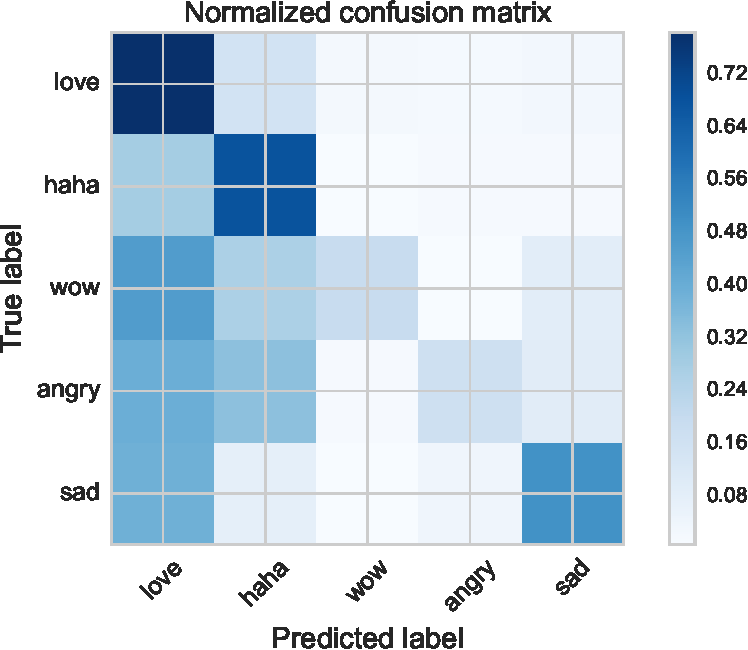
\includegraphics[width=0.9\columnwidth]{../3_notebooks/notebook_figures/conf.pdf}
\caption{Confusion matrix showing on what reactions the predictive model has trouble. The more intense the color blue, the more well-classified headlines.}
\label{fig:conf}
\end{figure}


\begin{table*}
\centering
\scriptsize 
\caption{Some predicted values, the first 10 are headlines not used in training, and the last ones are random headlines. $y_{\text{pred}}$ is the predicted reaction using the TF-IDF + Linear SVC model, $y_{\text{prob}}$ the sorted predicted probabilities per reaction using the TF-IDF + SGD model, and $y_{\text{true}}$ is the actual reaction.}
\label{tab:bla2}
\def\arraystretch{1.5}%  1 is the default, change whatever you need

\begin{tabular}{|>{\centering\arraybackslash}m{3cm}|c|c|c|}
\hline
\rowcolor{LightCyan} Headline & $y_{\text{pred}}$ & $y_{\text{prob}}$ & $y_{\text{true}}$ \\
\hline
Huma Abedin And Anthony Weiner Are Separating &       haha &   haha:0.519, sad:0.24, love:0.195, angry:0.0461, wow:0.0 &      haha:86, sad:77, love:38, wow:34, angry:4 \\
\hline
Apartment complex warns residents about clown trying to lure kids into woods &        sad &   sad:0.567, haha:0.19, love:0.171, wow:0.0712, angry:0.0 &  wow:1571, angry:770, sad:66, haha:58, love:28 \\
\hline
California Lawmakers Pass Bill Requiring Prison Sentence After Stanford Sex Assault Case &      angry &       angry:0.771, love:0.229, wow:0.0, sad:0.0, haha:0.0 &   love:1958, angry:751, wow:48, sad:42, haha:6 \\
\hline
Triumphant Tarantula Survives Being Eaten By Toad &        sad &   sad:0.357, haha:0.303, love:0.227, wow:0.114, angry:0.0 &  wow:1388, haha:382, love:156, sad:15, angry:5 \\
\hline
Scientists discover oldest fossils on Earth &        wow &     wow:0.996, sad:0.00439, love:0.0, haha:0.0, angry:0.0 &      wow:189, love:60, haha:15, sad:2, angry:2 \\
\hline
Wilderness Expert Finds A Giant Black Slug Which Is Way Bigger And Cooler Than You Thought | 9GAG.tv &       haha &    haha:0.527, wow:0.445, angry:0.0285, sad:0.0, love:0.0 &   wow:837, love:169, haha:144, sad:14, angry:1 \\
\hline
Georgia teacher dreams up dice game about slavery. It didn't go well. &       love &   love:0.855, haha:0.142, wow:0.00315, sad:0.0, angry:0.0 &      angry:107, wow:96, haha:42, love:9, sad:7 \\
\hline
Latino Trump Supporter Warns Of 'Taco Trucks On Every Corner' &       haha &  haha:0.486, love:0.238, angry:0.198, sad:0.0773, wow:0.0 &   haha:1524, love:231, wow:52, angry:30, sad:4 \\
\hline
Isis has nothing to do with islam &      angry &      angry:0.757, haha:0.243, wow:0.0, sad:0.0, love:0.0 & -\\
\hline
Justin Bieber is dead &       haha &    haha:0.61, sad:0.375, angry:0.0141, wow:0.0, love:0.0 & - \\
\hline
\end{tabular}
\end{table*}


%\section*{Acknowledgments}
%\appendix

\section{Conclusions}

We built a dataset of 9072 Facebook posts extracted from several fan-pages and from these posts we analyzed a text corpus of titles linking to a website. Then, we were able to discover features that can be used to obtain a good headline by considering the type of reaction it produces on people.

According to the results the most common reaction are ``haha'' and ``love''. These are more likely to produce more reaction votes and therefore become more popular. However, headlines that produce an ``angry'' reaction are more likely to produce more comments.

Among the headlines there were other types of content related with celebrities or news which mostly depends on the date the entry is published. A more specific type of content could produce better results, but it could is hard to find enough ``sad'' and ``angry'' reactions. 

It could be possible to obtain a better result by changing the parameters of the classifiers and feature models. Also, we tried mostly with BoW techniques, there should be a better way to extract features and considering the grammar structure. Moreover, sentiment analysis techniques could be used to get better assumptions on how to separate headlines by the type of reaction.

We dealt with a multi-class classification where the target takes one of 5 reactions, the highest or most voted reaction. We could have used the number of votes each of those reactions had as a discrete probability distribution. Finally, a deep learning approach might get a better performance.


% include your own bib file like this:
%\bibliographystyle{acl}
%\bibliography{acl2016}
\bibliography{acl2016}
\bibliographystyle{acl2016}

\appendix

\end{document}
